\section{}
Consider the following closed-loop system:
% too lazy to remake the block diagram with tikz
\begin{figure}[h]
    \centering
    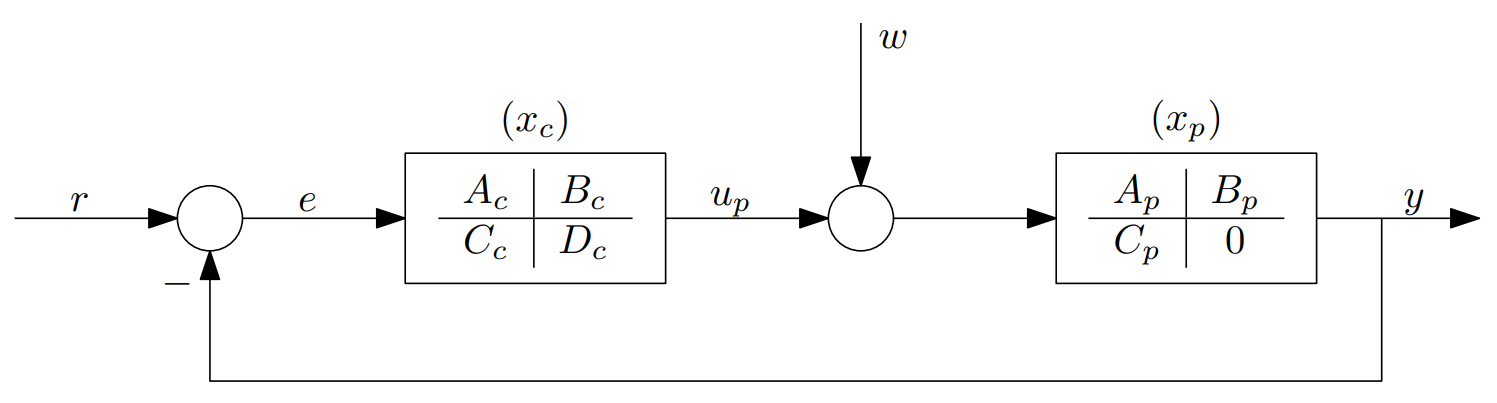
\includegraphics[width=0.5\textwidth]{Questions/Figures/Q3ProblemDiagram.png}
    \caption{Block diagram of the closed-loop system}
    \label{fig:Q3ProblemDiagram}
\end{figure}
The controller's state-space matrices are
\begin{equation*}
    A_c = -4, \quad B_c = 1, \quad C_c = -5, \quad D_c = 1
\end{equation*}
and the plant's are
\begin{equation*}
    A_p = \begin{bmatrix}
        0 & 1 \\
        -2 & -3
    \end{bmatrix}, \quad
    B_p = \begin{bmatrix}
        1 \\
        0
    \end{bmatrix}, \quad
    C_p = \begin{bmatrix}
        1 & 0
    \end{bmatrix}
\end{equation*}
\begin{enumerate}[label=(\alph*)]
    \item Form the closed-loop system dynamics matrix $A_{cl}$. Verify the internal stability of the system.
    \item Convert the state-space control and plant blocks into transfer functions $G_c(s)$ and $G_p(s)$, then form the characteristic polynomial. Verify the input-output stability of the system (note you can either compute the roots numerically, or use the Routh-Hurwitz criterion)
    \item What's the relationship between the results in (a) and (b)?
\end{enumerate}

\subsection{}
% \subsection{Closed Loop Stability}
% \begin{figure}[h]
%     \centering
%     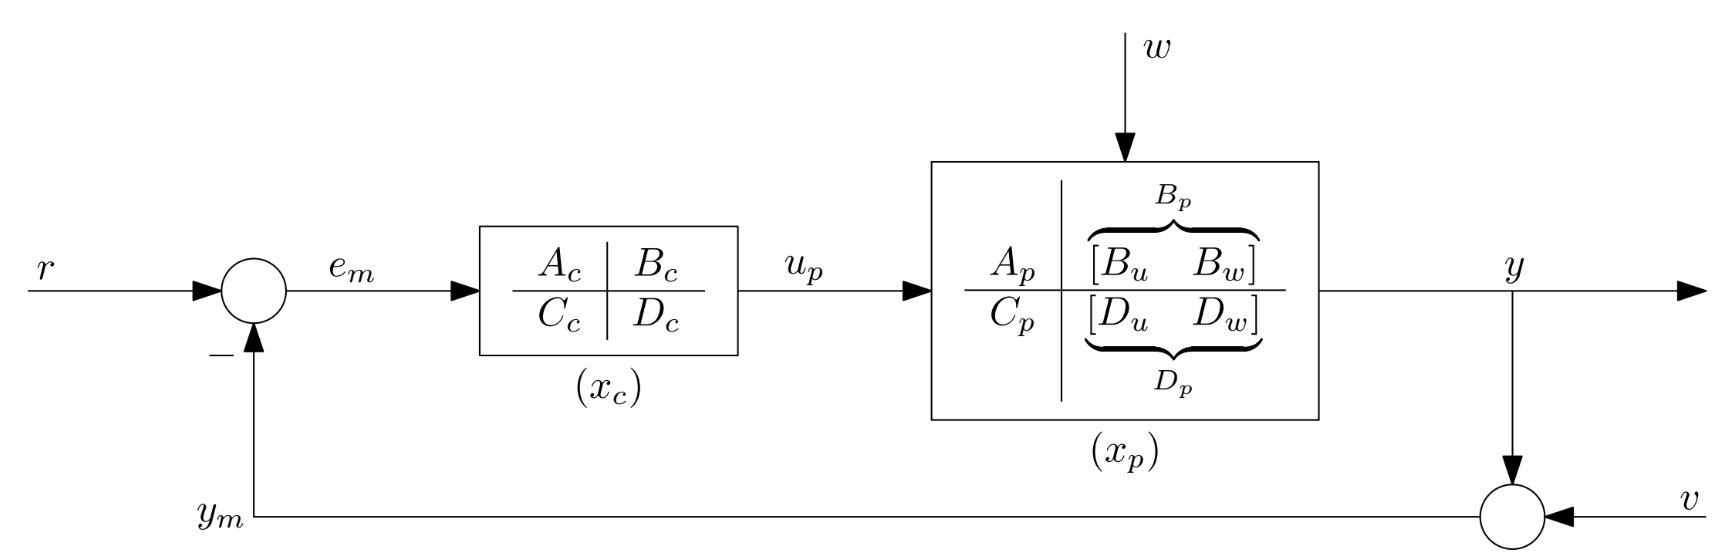
\includegraphics[width=0.5\textwidth]{closed loop diagram.png}
%     \caption{Closed loop system}
% \end{figure}
% Assume:
% \begin{itemize}
%     \item Both controller ($A_c$, $B_c$, $C_c$, $D_c$) and plant ($A_p$, $B_p$, $C_p$, $D_p$) are minimal realizations.
%     \item $D_c= 0$ or $D_p = [D_u, D_w] = 0$, such that $D_c D_u = D_u D_c = 0$ and $D_c D_w = D_w D_c = 0$.
% \end{itemize}
% Then, the state-space form of the closed loop system is:
% \begin{align*}
%     \dot{x}_cl &= \begin{bmatrix}
%         \dot{x}_c \\
%         \dot{x}_p
%     \end{bmatrix} = \underbrace{
%     \begin{bmatrix}
%     A_c - B_c D_u C_c & -B_c C_p \\
%     B_u C_c & A_p - B_u D_c C_p
%     \end{bmatrix}}_{A_{cl}}
%     \begin{bmatrix}
%         x_c \\
%         x_p
%     \end{bmatrix} + \underbrace{
%     \begin{bmatrix}
%         B_c & -B_c D_w & -B_c \\
%         B_u D_c & B_w & -B_u D_c
%     \end{bmatrix}}_{B_{cl}}
%     \begin{bmatrix}
%         r \\
%         w \\
%         v 
%     \end{bmatrix} \\
%     y_cl &= \begin{bmatrix}
%         e_m \\
%         u_p \\
%         y  \\
%         y_m 
%     \end{bmatrix} = \underbrace{
%     \begin{bmatrix}
%         -D_u C_c & -C_p \\
%         C_c & -D_c C_p \\
%         D_u C_c & C_p \\
%         D_u C_c & C_p 
%     \end{bmatrix}}_{C_{cl}}
%     \begin{bmatrix}
%         x_c \\
%         x_p
%     \end{bmatrix} + \underbrace{
%     \begin{bmatrix}
%         1 & -D_w & -1 \\
%         D_c & 0 & -D_c \\
%         0 & D_w & 0 \\
%         0 & D_w & 1
%     \end{bmatrix}}_{D_{cl}}
%     \begin{bmatrix}
%         r \\
%         w \\
%         v
%     \end{bmatrix}
% \end{align*}
To be able to use the developments in the notes, two assumptions have to be satisfied:
\begin{itemize}
    \item Both controller ($A_c$, $B_c$, $C_c$, $D_c$) and plant ($A_p$, $B_p$, $C_p$, $D_p$) are minimal realizations.
    \item $D_c= 0$ or $D_p = [D_u, D_w] = 0$, such that $D_c D_u = D_u D_c = 0$ and $D_c D_w = D_w D_c = 0$. This is satisfied in this case, since $D_p = 0$.
\end{itemize}
Then, the state-space form of the closed loop system is calculated by Matlab:
\begin{verbatim}
>> Gc
 
Gc =
 
1 - 5/(s + 4)
 
>> Gp
 
Gp =
 
(s + 3)/(s^2 + 3*s + 2)
\end{verbatim}

Both $G_c(s)$ and $G_p(s)$ are minimal realizations, so the derivations in the notes can be used.
\begin{align*}
    A_cl = \begin{bmatrix}
        A_c & -B_c C_p \\
        B_u C_c & A_p - B_u D_c C_p
    \end{bmatrix} 
\end{align*}
Employing Matlab again,
\begin{verbatim}
Acl =

    -4    -1     0
    -5    -1     1
     0    -2    -3


V =

   -0.5774    0.2145    0.1345
   -0.5774   -0.7762   -0.1859
   -0.5774    0.5929    0.9733


D =

   -5.0000         0         0
         0   -0.3820         0
         0         0   -2.6180

Real part of eigenvalues of Acl: 

ans =

   -5.0000         0         0
         0   -0.3820         0
         0         0   -2.6180
\end{verbatim}

\textbf{Since all the eigenvalues of $A_{cl}$ have negative real parts, the closed-loop system is internally stable.}

All Matlab calculations can be found in the script:
\lstinputlisting[language=Matlab]{Questions/Code/a6q3a.m}